%18/09 - Patricia Álvarez
\chapter{Cronogramas - árboles temporales}
Para estimar los años o las fechas de los cambios evolutivos de los caracteres se emplean cronogramas. La datación se basa en el reloj molecular, que a su vez se basa en la tasa de evolución de diferentes macromoléculas, ya sea ADN o proteínas. Se propone que las tasas evolutivas son constantes en el tiempo. Cada proteína o cada gen es un reloj independiente; aunque la tasa sea constante para los linajes, no es igual para todos los genes o proteínas. Para la calibración de la datación se utiliza la fecha de muestreo, la edad del fósil y los eventos biogeográficos (eventos geológicos, como apertura o cierre de océanos, movimiento de continentes, etc). Para crear estos árboles, al programa se le aportan unas estimaciones temporales, que pueden ser más estrictas (strict clock) o más relajadas (relaxed clock). Como mínimo, se debe tener una datación para el grupo externo. 

\begin{figure}[htbp]
\centering
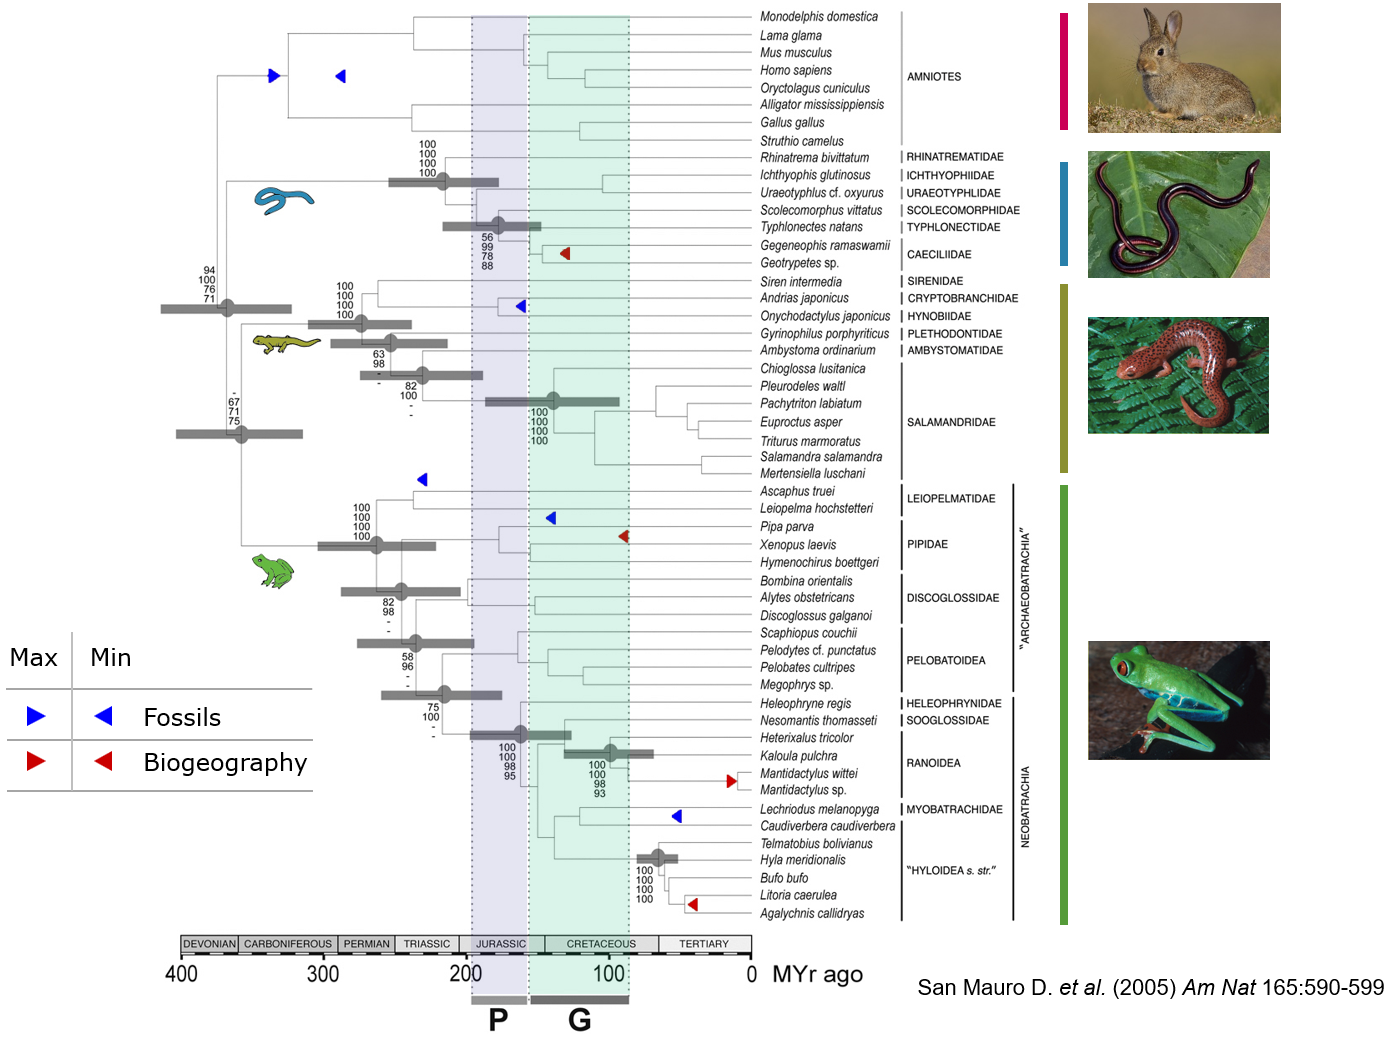
\includegraphics[width=0.9\linewidth]{figs/cronograma-ejemplo.png}
\caption{Ejemplo de cronograma. La datación se ha basado en registros fósiles (flechas azules) y eventos biogeográficos (flechas rojas).}
\end{figure}